\section*{Inversion problems, recent solutions and limitations}

The non-destructive test in sublayers identification as well as other size characterization purposes has been used for several decades. The non-destructive methods are cost effective and time efficient (Tomeh et al., 2006) such as spectral analysis of surface waves (SASW), multichannel analysis of surface waves (MASW), those methods are the most popular surface wave methods employing the properties of wave propagation of Rayleigh waves and Love waves in soil media  (Kallivokas et al., 2013; C. P. Lin et al., 2017; C. P. Lin \& Chang, 2004; Mahvelati et al., 2017; Park et al., 1999; Penumadu \& Park, 2005; Xia et al., 1999). 

The process of waveform inversion is to transform in-situ geophysical parameters into engineering parameters. Different techniques have been introduced for the inversion analysis such as first arrival method or dispersion curve approach. Dispersion is one of the important properties of wave travelling in solid medium, in which the relationship of angular frequency and the wave number is non-linear or different frequency components travel at different speeds (the group velocity component travels faster or slower than the phase velocity). Using the dispersion curve, the wave parameters can be used to transform to infer the layer profile. The inversion of geophysical properties of soil layers to the geotechnical properties known as inversion problems has been studying for many years and there are various inversion models proposed to invert the seismic wave field to the shear velocity profile and other geotechnical parameters such as horizontal to vertical spectral ratio (HVSR) (Deren Yuan \& Nazarian, 1993; García-Jerez et al., 2016; Kallivokas et al., 2013; Leong \& Aung, 2013; Luke et al., 2007; Moro, 2015b; Olafsdottir et al., 2020; Thorson \& Claerbouts, 1985; Wathelet et al., 2004). The application of surface wave analysis for soil characterization is large such as ground improvement quality assessment, underground object detection, (Abudeif et al., 2019; Chris King et al., 1989; Sebastiano Foti et al., 2011; C.-P. Lin et al., 2012; C. H. Lin et al., 2017; Matthews et al., 2000; Tran et al., 2014). 

 However, the inversion problems are very complicated because of the uncertainties of the field conditions, data collection operations and many other impacts which contribute to make the non-uniqueness of inversion results (S. Foti et al., 2009; Roy \& Jakka, 2017, 2018; Williams \& Penumadu, 2011). The non-uniqueness of the inversion result is the reason making non-destructive surface wave methods be less reliable and conventional methods such as borehole tests, cone penetration test (CPT), standard penetration test (SPT) and other techniques. One of the common situations of non-uniqueness inversion is the occurrence of different shear wave velocity profiles of a certain inversion model or the similar shear wave velocity with the very different HVSR graphs. There are plenty of factors that influence the variation of the expected inversion results (nearest offset, geophone spacing, geophone spread length, field conditions, test equipment, testing time and other indicators).
 
A research on the use of middle-of-receiver-spread assumption of MASW method (Luo et al., 2009) indicated that the results of dispersion curves are very similar with the different nearest offset, and the dispersion curves are more likely to be different under the change of receiver spread structure. The above technique presents a method to explore the factors that are most likely to cause the non-uniqueness phenomenon in inversion problems. There are various indicators that cause non-uniqueness such as the data is inadequate, the complexity of site conditions, the coarse model characterization, or the model parameterization is not proper. A study on the inversion of seismic surface wave in case of complex profiles (Luke et al., 2007) presented a model to deal with a non-uniqueness problem adopting a two-step process, which is first optimizing model parameters by imposing searching boundaries, and then using the process of stochasticity with a large number of iterations to converge to the results with acceptable confidence level. 

It is the higher-order modes that make uncertainty in choosing proper orders to invert. Therefore, many efforts aim to solve the non-uniqueness of inversion problems including the conventional inversion, the statistical, image processing, and neural network approaches. The interpretation of inversion results in very important, because the outcomes may not be used until one could properly explain his or her data and inversion model. In surface wave analysis, the results of inversion are usually the phase velocity profile, sublayer identification, compressional velocity profile (less common), the horizontal to vertical spectral ratio. The process of inversion is usually complicated involving data acquisition, dispersion analysis and the inversion techniques are applied. In the inversion problem, the introduction of parameterization and the use of standardization are very important to avoid the non-uniqueness of the inverted results. Nevertheless, the regularization and standardization of the use of geophysical test methods to apply to derive geotechnical engineering parameters are still quite limited, the international standards related to seismic tests are Cross-hole Method (ASTM D4428/D4428M-14, 2014), Down-hole Method (ASTM D7400/D7400M-19, 2019), Seismic-Reflection Method (ASTM D5777-18, 2018), Seismic-Refraction Method (ASTM D5777-18, 2018), Geotechnical Borehole Geophysical Logging (ASTM D5753-18, 2018), the guide for selecting geophysical methods (ASTM D6429-20, 2020) and others. 
 
The inversion problems involve three main works which are (1) field data acquisition; (2) dispersion analysis; and (3) inversion. There are various data acquisition techniques (Moro, 2015a). Generally, the general surface wave tests are the passive methods and the active methods, the dispersion analysis methods has been studying and different techniques have been proposed such as the tau-p transformation (George A. McMechan \& Mathew J. Yedlin, 1981), f – k transformation, phase-shift method (Choon Byong Park et al., 1998) and the stacking method (Thorson \& Claerbouts, 1985; Xia et al., 2007), and the image processing-based technique employing threshold energy filtering of the dispersion image (Taipodia et al., 2020). The use of two receivers to test and analyze the dispersion curve by SASW method is applicable and it takes the advantage of the large spreading, but it also has drawbacks related to the mode jumping in the dispersion curve images (Osama AI-Hunaidi, 1994). Other methods of dispersion analysis have also been studied with disadvantages and pitfalls, the attention on the multiple modes in dispersion analysis is much more common (Hayashi, 2012; C. P. Lin \& Chang, 2004; Supranata et al., 2007).    
 
Some studies pointed out that the properties of the dispersion curve may not only rely on the fundamental mode phase velocity of the dispersion curve, but also high modes phase velocity dispersion curves, which means that the different modes may contain the sublayers’ information at different depths. The studies on using the combination of several modes of dispersion, the technique is so-called the effective dispersion curve of the apparent dispersion curve (Olafsdottir, Bessason, et al., 2018; Osama AI-Hunaidi, 1994; Subramaniam et al., 2020; Supranata et al., 2007). 






\section*{Artificial neural networks and its applications in geophysical problems}

There are also plenty of studies on the application of DL and ML in geophysical problems (Diersen et al., 2011; Guo, 2021; Liu et al., 2020; Peters et al., 2019; Ross et al., 2018; Wilkins et al., 2020; Zhang et al., 2020). A study on the P-wave arrival picking and the first motion polarity determination with deep learning (Ross et al., 2018) indicated that the automated algorithm for estimating the P-wave arrival has been less precise than the performance of human experts. However, dealing with a large scale, human efforts are impossible, therefore a CNNs has been proposed to use the datasets which are from the human experts’ dataset (millions of pictures from experts’ picking) and training the data for future prediction. The result indicated that the CNNs predict with the precision up to 95 percent compared to that of experts’ picking data. A recent study on Automatic picking of multi-mode surface-wave dispersion curves based on machine learning clustering methods (Wang et al., 2021) proposed method of automatic picking method of multiple-mode surface wave dispersion curves employing an unsupervised learning approach. The 2D dispersion images are used as input data, clustering the dispersion energy and the background noise is performed. Then the multi-mode dispersion curves are identified by searching algorithm for local peaks, then the noise is removed by the particle filter. The results show that the automatic pick dispersion curves match the theoretical dispersion curves. The automatic pick dispersion curves are used in inversion problems and the result indicates an agreement with the borehole data. 

Those above studies have demonstrated that the application of DL and ML are very powerful and potential in inversion problems. The results of previous studies have also presented that the use of DL and ML for inversion are well matched with the geotechnical test.

A research on Deep learning and process understanding for data-driven Earth system science (Reichstein et al., 2019), the study stated that machine learning approaches are developed and used popularly to extract patterns and insights from geophysical data. In the paper, it is argued that the deep learning approach should be employed rather than the classical machine learning, such that the approach enables automatic extraction of special features to gain more understanding of the earth system, improving prediction ability and interpretability of earth structure.

\begin{figure}
    \centering
    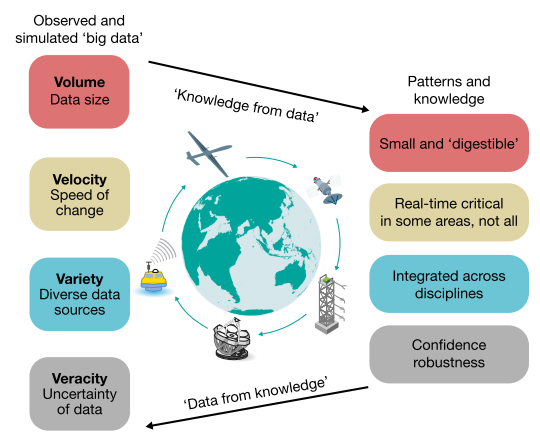
\includegraphics[scale=0.5]{images/bigdata.png}
    \caption{Big data challenges in the geoscientific context (Reichstein et al., 2019).}
    \label{fig:bigdata}
\end{figure}


Figure \ref{fig:bigdata} presents the big data involving the concept of “four Vs”, including volume, velocity, variety and veracity. The key is to overcome the challenges of the capability of extracting the interpretable information and the knowledge from big data. Unfortunately, our ability to collect and create data outpaces our ability to properly interpret it. The capability to explain the data over the last few decades has not been at the same rate with the data available. It has been recognized that, to get the meaningful part from big data, we may need to cope with two main tasks, which are (1) to extract the knowledge from data, and (2) building models that learn from the data much more from the traditional data assimilation approaches, but still respect the nature’s law.


\begin{figure}
    \centering
    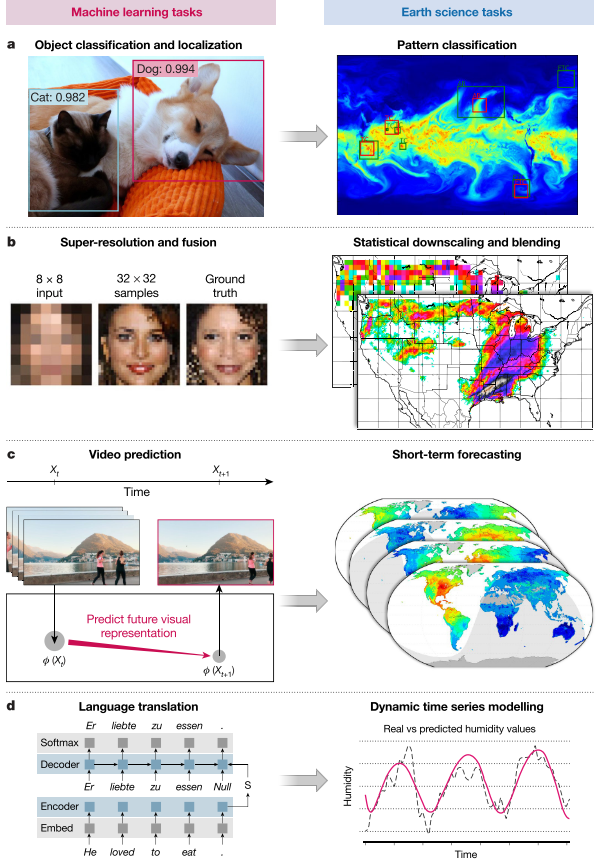
\includegraphics[scale=0.6]{images/MLapp.png}
    \caption{Four examples of typical deep learning applications (left panels) and the geoscientific problems they can be applied to (right panels) (Reichstein et al., 2019).}
    \label{fig:MLapp}
\end{figure}

Although the intensive studies and widely sheared deep artificial neural networks, the similarity between the traditional machine learning and applied machine learning in the field of geophysics is striking, but still need a lot of works need to be done to really understand and apply properly machine learning in the field. The examples of the similarity between traditional machine learning model and the use of machine learning in the field of geophysics are shown in figure \ref{fig:MLapp}, the linkages between the physical models and machine learning is abstractly illustrated in figure \ref{fig:MLarchi}.


\begin{figure}
    \centering
    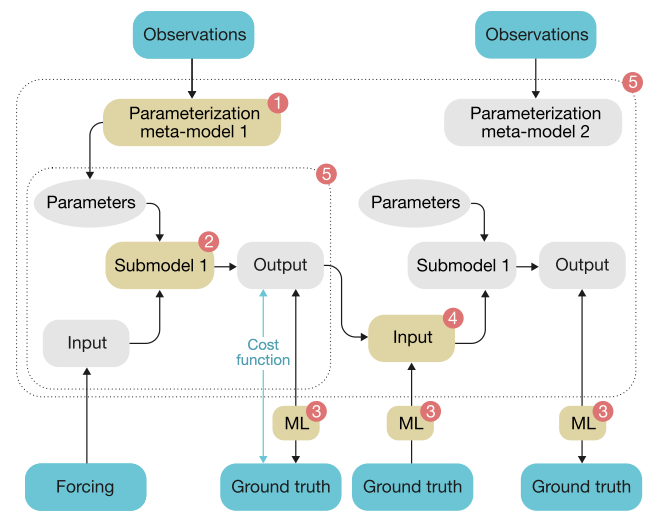
\includegraphics[scale=0.6]{images/MLarchi.png}
    \caption{Linkages between physical models and machine learning}
    \label{fig:MLarchi}
\end{figure}


A study on a deep residual network of convolution and recurrent units for earthquake signal detection (Mousavi et al., 2019) that makes use of combination of convolution layers and bi-directional long-short-term memory units in a residual structure. The model learns from the time-frequency properties of earthquake signals of three component data with different station data collection. The network is trained with 500, 000 seismograms taken in Northern California. The network architecture is shown in figure \ref{fig:NNarchi}, which includes four main parts (1) seismograms input, (2) feature extraction, (3) sequential learning, and (4) classification.   


\begin{figure}
    \centering
    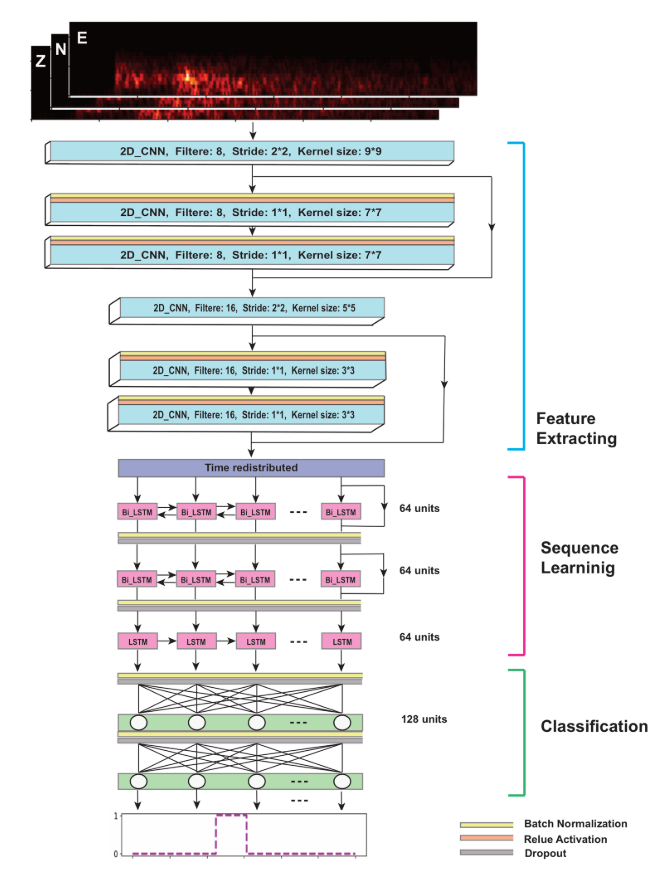
\includegraphics[scale=0.6]{images/NNarchi.png}
    \caption{The architecture of our proposed deep neural network (Mousavi et al., 2019)}
    \label{fig:NNarchi}
\end{figure}

The architecture of the network is presented to include three types of layers: (1) convolution layers, (2) recurrence layers, and (3) and the fully connected layers. The description of the training and testing data dataset is that there is 80 percent data for training, 10 percent data for validation and the final 10 percent is the testing data. The optimization model used is Adam, the number of epochs is 62. 


\begin{figure}
    \centering
    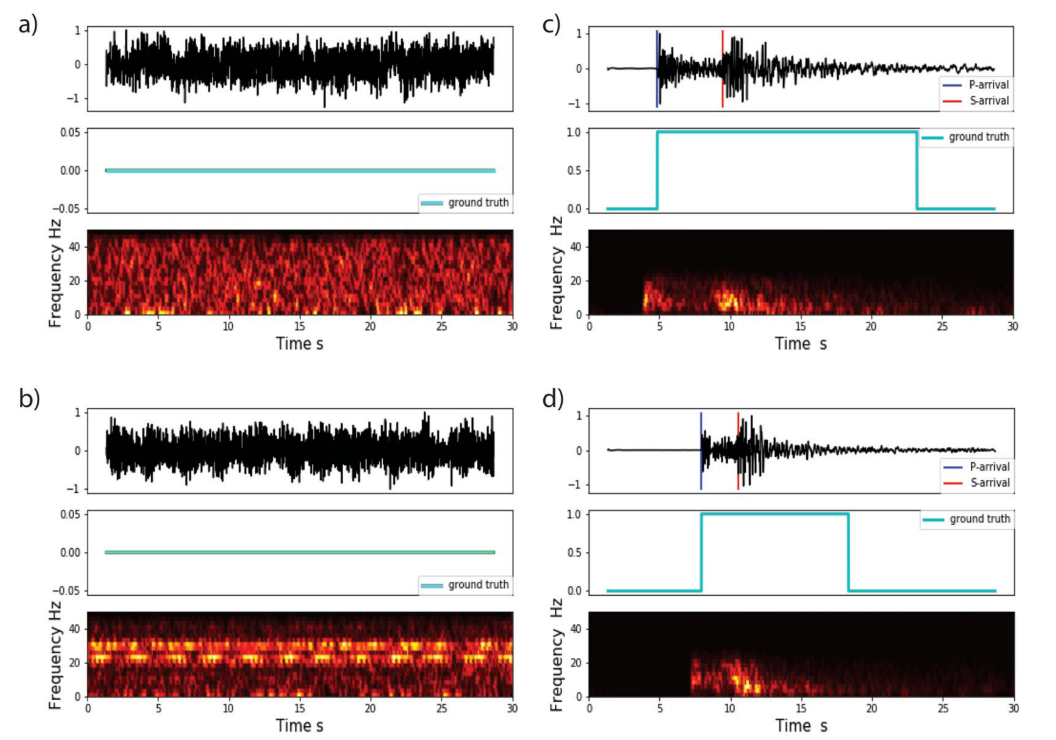
\includegraphics[scale=0.4]{images/seisEX.png}
    \caption{Examples of seismographs, label vector, and associated spectrogram (short time Fourier transform, STFT) for vertical components of two sample noises (a,b) and two earthquake samples (c,d) (Mousavi et al., 2019)}
    \label{fig:seisEX}
\end{figure}

The results of the previous study indicated that the proposed network is reliable and efficient, the framework has the great expectation for reducing the detection threshold while minimizing false passive detection rates. 

\section*{Problem definition}

Although various conventional inversion models have been introduced and used wildly all over the world, people are still facing the uncertainties and non-uniqueness of the data and inverted results. The use of such an inversion model may need a lot of evaluations and judgements of experts who have much experience dealing with inversion problems.

The recent development of waveform inversion approaches brings to engineers many beneficial aspects. Because the conventional inversion process inevitably produces a lot of information, such as measurement of waveforms should be fully utilized to maximize the information content for inversion (i.e., full waveform and holistic approach). Those can be the data for the artificial neural networks (such as RNNs, CNNs, and GANs). The information extracted from the conventional inversion approaches can be full-wavefield seismograms, pre-processed wavefields, dispersion images, spectral ratio (HVSR, HVPD). As we have more information, we may be able to improve the resolution and accuracy of inversion results (such as velocity profiles, Poisson ratio profiles).

One more problem that we may face when dealing with conventional inversion is time consuming. Some models require much time to process. Utilizing neural networks means that machine learning and deep learning will play the role of extracting necessary information. Thus the quantity of data can be reduced, but still contain much meaningful data. 

\section*{Proposed methodology}

The method we propose is the application of a neural network, we would like to call it the inversion neural network. This method requires data for training the network to let the network learn to extract the features of input data which are the dispersion images, images of spectral ratio and other data from pre-processing stage. In this stage, we need to find a good automated inversion method to generate data for training later. The conventional inversion methods are used and compared and we will need to choose a specific inversion technique that is more robust.

The idea of inversion-based images is the use of data from realistic numerical models and treated them as images, then data in form of images will be the input vectors of the ANNs (Convolution Neural Networks, Recurrence Neural Networks, Generative Adversarial Networks or other new developed networks). The whole data is generally divided into three parts (training data, validation data, and test data), the training data and validation data are involved first and the test data involved in the end. The training process consumes most of the time (it is like human learning process), after each cycle of training, the validation data will come to evaluate whether the training data is good or not (this is based on the accuracy and the error cures). After training, the prediction will come to predict the new data (test data) based on the trained data. An example of CNN architecture is shown in figure \ref{fig:CNN}, the figure is taken from the Mathworks. 


\begin{figure}
    \centering
    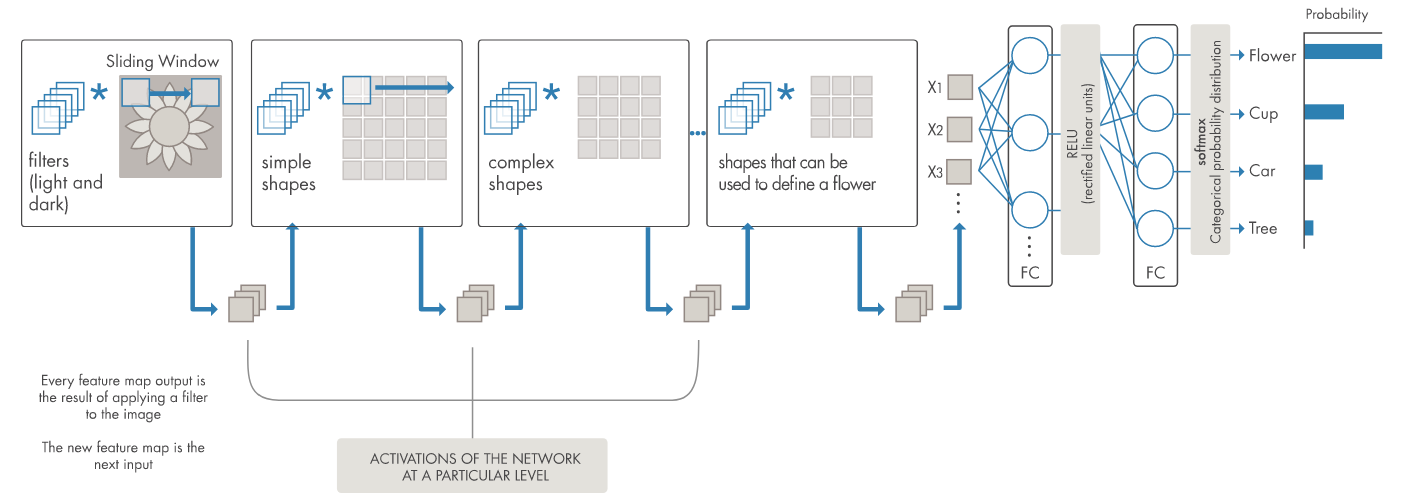
\includegraphics[scale=0.4]{images/CNN.png}
    \caption{Illustration of a CNN (courtesy of Mathworks)}
    \label{fig:CNN}
\end{figure}

The network initialization (input, initial weight, initial bias), architecture and other hyper-parameters (number of nodes, number of layers, activation functions, gradient descent scheme, number of epochs, …) are defined by the one who is working with it. The model is designed to consist two parts, the first stage is manually extractions of objective features from the data using Machine Learning algorithm available and the second stage is the fully connected network with a set of layers (input layer, convolution layers, pooling layers, classification layers, fully-connected layer, Softmax layer, …) and activation functions figure \ref{fig:activatefun} (Linear, ReLU, Sigmoid activation functions). 



\begin{figure}
    \centering
    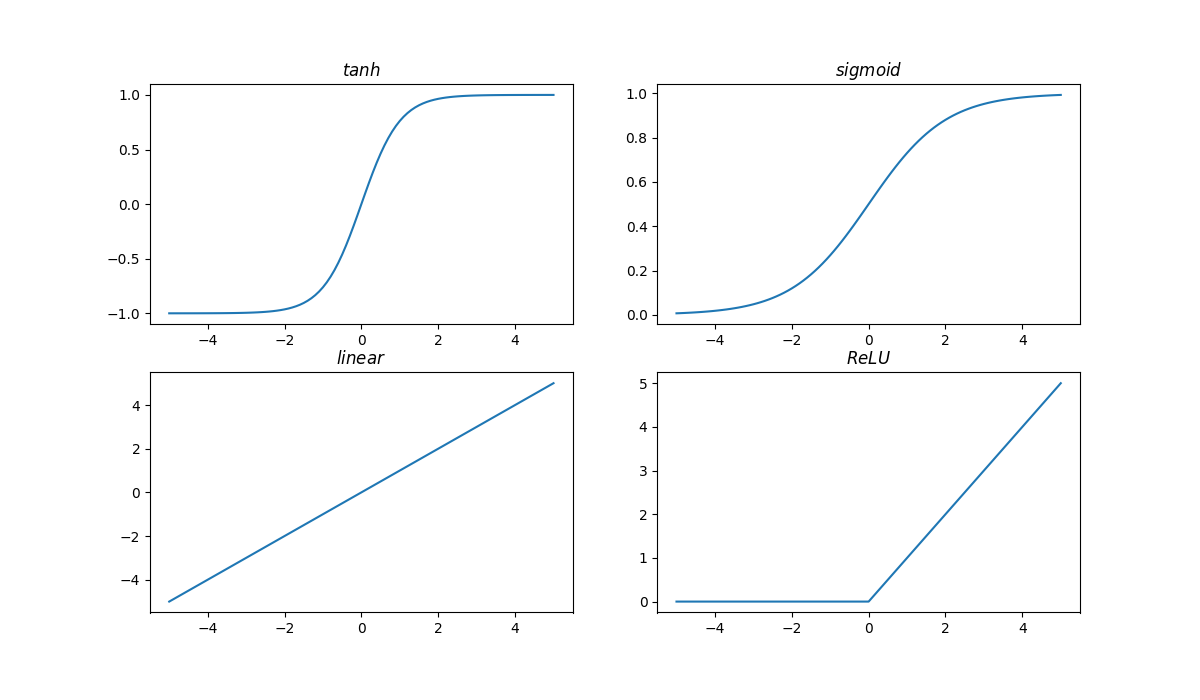
\includegraphics[scale=0.3]{images/activatefun.png}
    \caption{Some of popular activation function}
    \label{fig:activatefun}
\end{figure}


After the classification or prediction is done, the test data is involved to measure the misfit of the prediction, the test data is considered as the true answers (or the expected ground truth), then after error evaluation, the model will adjust its parameters to improve the performance based on the very famous method of “back-propagation” employing available algorithms (Stochastic Gradient Descent (SGD), SGD with momentum, Adam, RMSProp, …).        

Because the problem has unknown ground truth in nature. It is different from the popular faces, hand-written digits or objects recognition problems which were studied several decades ago and still popular recently. We do not know yet the true answers, the real data will naturally come from the traditional geotechnical field test (borehole samplings, in-situ subsurface parameters exploration), geophysical explorations (cross hole, down hole, surface wave methods, and even electrical methods), and data are then pre-processed, processed using developed numerical models to extract the information from the raw data. From those extracted features (such as dispersion curves of horizontal/radial and vertical components, RVSR, RVPD and other field data that are applicable).

Figure \ref{fig:inversionprocedure} illustrates the overview of the MASW method (Olafsdottir, Erlingsson, et al., 2018). The data is collected and the presentation of data in form of seismograms, the dispersion curve analysis and the inversion.

\begin{figure}
    \centering
    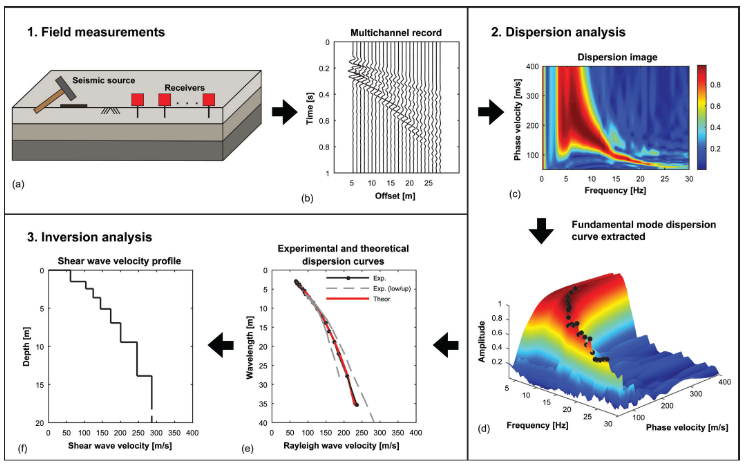
\includegraphics[scale=0.5]{images/inversionprocedure.png}
    \caption{SOverview of the MASW method: (a, b) field measurements; (c, d) dispersion analysis; (e, f) inversion analysis (Olafsdottir, Erlingsson, et al., 2018)}
    \label{fig:inversionprocedure}
\end{figure}

The data collection from available sources and the field acquisition data are used for both conventional inversion problems (concentrate on full-wavefield inversion) and the artificial neural networks (concentrate on convolutions neural networks). The data used in conventional inversion and CNNs are from the surface wave test (MASW). 

Pre-processing (i.e., remove mean, data normalization) may be necessary, the data input of CNNs are dispersion curve or spectral ratio of horizontal and vertical velocity components. The dispersion analysis is required; the extraction of fundamental mode dispersion curve or higher-order dispersion curves is used for the input of the inversion process. In CNNs model the data is divided into three parts, which include:
(1) Training data;
(2) Validation data;
(3) Test data.
The proportion of each part is selected based on the suggestion of previous research or can be chosen randomly with the higher proportion of training data (around 80 percent) and lower proportion of validation (around 10 percent) and test data (around 10 percent). The performance of conventional inversion process involving three main parts, which are:
(1) data acquisition; 
(2) dispersion analysis;  
(3) inversion.
It is very crucial to notice that we do not have data at hand, we need to prepare the fairly large amount of data for training the network. The proposed training information is the dispersion images, feature images (horizontal-to-vertical spectral ratio images) and the shear wave velocity profiles (labels). To have this data, we need to have a inversion algorithms that can automatically perform inversion analysis that are reliable and need to be validated with other proposed algorithms. Once we have the data set at hand, we then could be able to use it the training the inversion networks. This is considered as supervised learning approach.

\begin{figure}[!t]
    \centering
    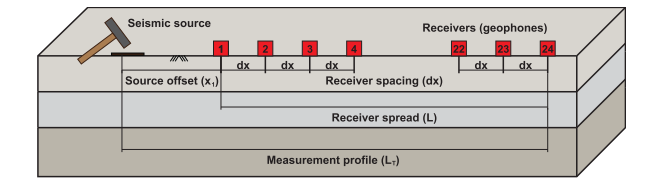
\includegraphics[scale=0.6]{images/geophoneconfig.png}
    \caption{Typical MASW measurement profile (Olafsdottir, Erlingsson, et al., 2018)}
    \label{fig:igeophoneconfig}
\end{figure}


\begin{figure}[!t]
    \centering
    \begin{subfigure}[b]{0.45\textwidth}
        \centering
        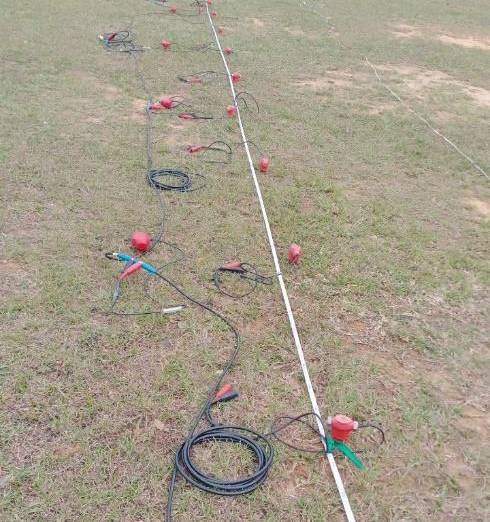
\includegraphics[width=\textwidth]{images/fieldtesta}
        \caption{Testing field}
        \label{fig:fieldtesta}
    \end{subfigure}
    \hfill
    \begin{subfigure}[b]{0.45\textwidth}
        \centering
        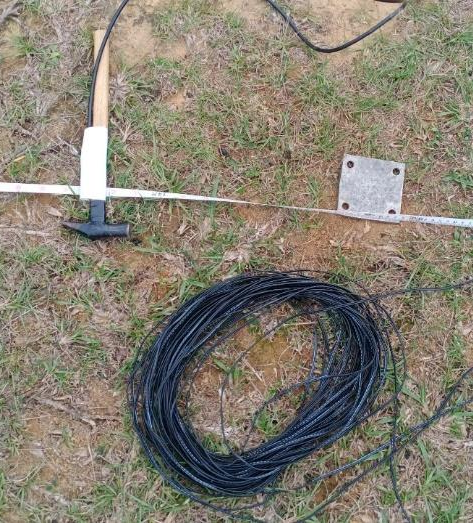
\includegraphics[width=\textwidth]{images/fieldtestb}
        \caption{Mini hammer}
        \label{fig:fieldtestb}
    \end{subfigure}
    \hfill
    \begin{subfigure}[b]{0.45\textwidth}
        \centering
        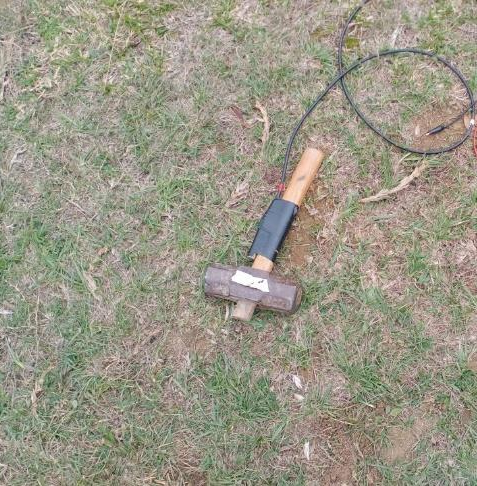
\includegraphics[width=\textwidth]{images/fieldtestc}
        \caption{Small hammer}
        \label{fig:fieldtestc}
    \end{subfigure}
    \hfill
    \begin{subfigure}[b]{0.45\textwidth}
        \centering
        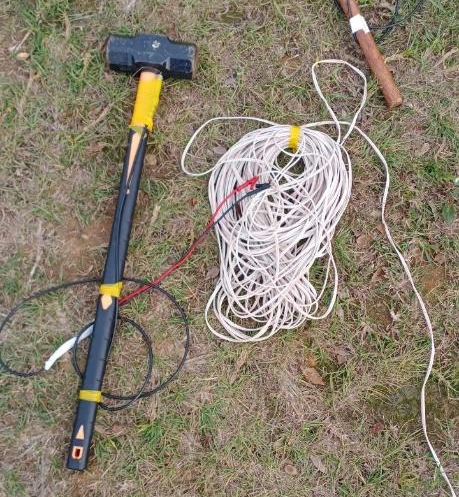
\includegraphics[width=\textwidth]{images/fieldtestd}
        \caption{Big hammer}
        \label{fig:fieldtestd}
    \end{subfigure}
    \hfill
    \caption{Illustrations of testing location and sources types}
    \label{fig:fieldtest}
\end{figure}    


\begin{table}
  \centering
  \caption{MASW Experiment parameters}
  \setlength{\tabcolsep}{4pt}
  \renewcommand{\arraystretch}{1.2}
  \begin{tabu}{*{8}{X[c]}}
  \toprule
        \multirow{2}{*}{\textbf{Parameters}} & \textbf{Dimension} & \multicolumn{3}{c}{\textbf{Vertical geophones}} & \multicolumn{3}{c}{\textbf{Horizontal geophones}} \\ \cline{2-8}
        & \textbf{Types} & \textbf{Mini} & \textbf{Small} & \textbf{Big} & \textbf{Mini} & \textbf{Small} & \textbf{Big} \\ 
  \midrule
        X_0 & m & 1 & 3 & 10 & 1 & 3 & 10 \\ 
        \delta x & m & 1 & 1 & 1 & 2 & 2 & 2 \\ 
        Stacking & Times & 5 & 3 & 4 & 5 & 3 & 3 \\ 
        ID & - & 3237 & 3240 & 3239  & 3242 & 3241 & 3243 \\ 
        Name & - & V(mini) & V(small) & V(big) & V(mini) & V(small) & V(big) \\ 
        Name & - & ch10,flip & ch10,flip & ch10 & ch10 & ch10 & 10,flip \\ 
  \bottomrule
  \label{tab:fielddata}
  \end{tabu}
\end{table}

\begin{figure}
    \centering
    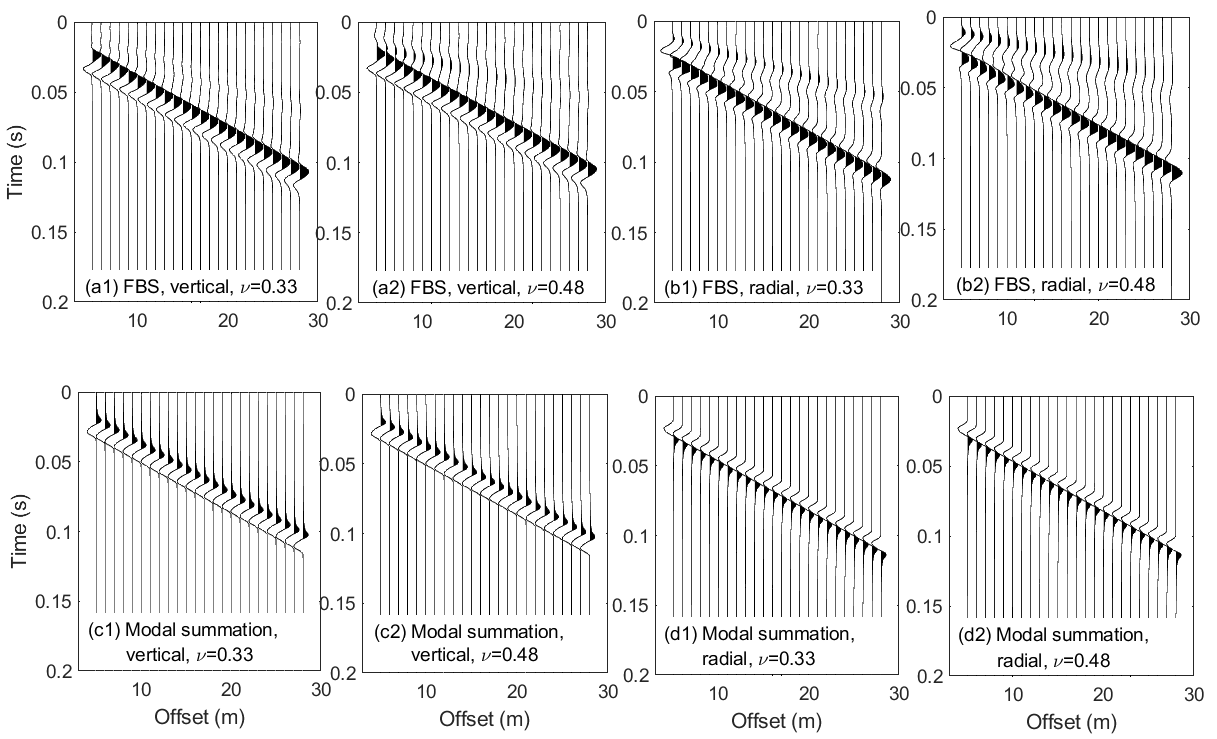
\includegraphics[scale=0.45]{images/wavefield.png}
    \caption{Synthetic seismograms of the homogeneous model with different Poisson’s ratio Poisson's ratio using the FBS approach (top, (a) for vertical and (b) for radial component) and the modal summation method (bottom, (c) for vertical and (d) for radial component). (Courtesy of Lin and his reesarch lab)}
    \label{fig:wavefield}
\end{figure}

There are some algorithms that are considered to perform the inversion, they are framework of full-wavefield inversion based on the Fourier-Bessel expansion, fast inversion (Cao et al., 2011), simplified inversion (Pelekis \& Athanasopoulos, 2011). The CNNs also involve three main parts, which are (1) data input; (2) training data and (3) prediction 

The input or input layer will be the image dataset from numerical models including dispersion curves, RVSR images, RVPD images shown in figure \ref{fig:DCinput} and figure \ref{fig:RVSRinput}.


\begin{figure}[!t]
    \centering
    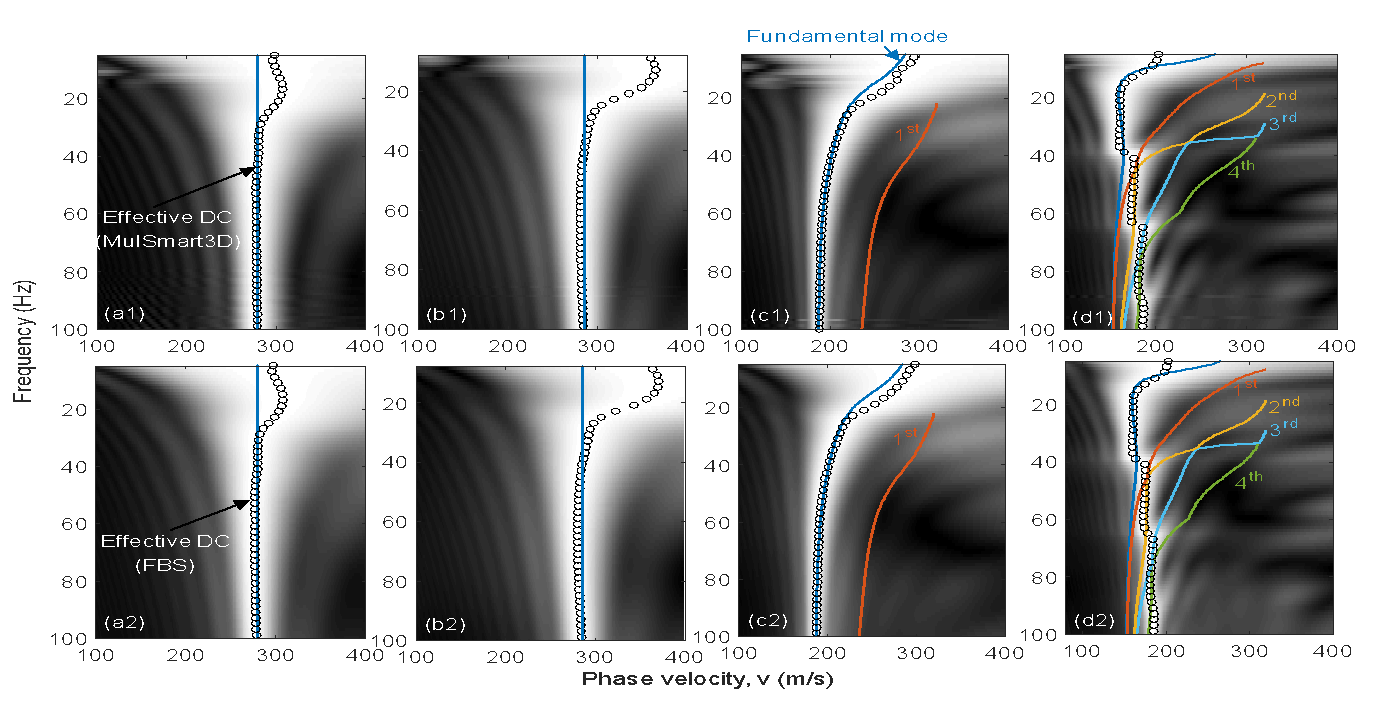
\includegraphics[scale=0.3]{images/DCinput.png}
    \caption{Look at dispersion images as input data (seismic features)}
    \label{fig:DCinput}
\end{figure}


\begin{figure}[!t]
    \centering
    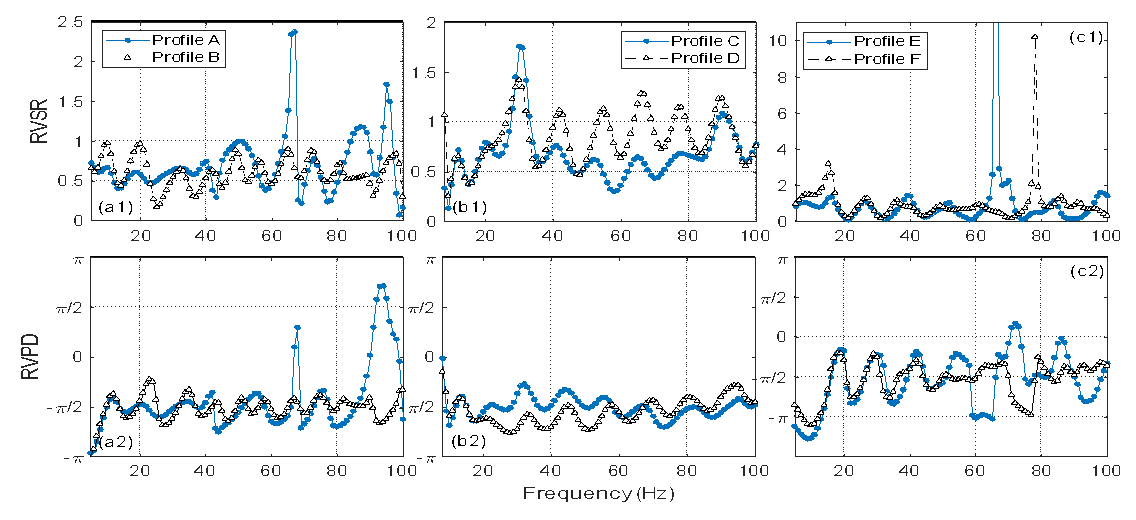
\includegraphics[scale=0.5]{images/RVSRinput.png}
    \caption{Look at SRVSR and RVPD as input data (seismic features)}
    \label{fig:RVSRinput}
\end{figure}

An illustration of field data acquisition as an example of data collection. The test was taken in the Softball field located at National Yang Ming Chiao Tung University, survey length is 23 m. The geometry design of the field test Figure 16, the testing location and types of hammer (impulse generators) are shown in Figure 17, the testing information and field description are presented in table \ref{tab:fielddata}, the synthetic seismograms are presented in figure \ref{fig:wavefield}.

The network hyper-parameters are chosen and adjusted to find the most appropriate network architecture for the performance of prediction, and avoid problems such as being stuck in local minima, overfitting or underfitting. The performance of both conventional inversion and inversion applying CNNs are judged and compared. 

\section*{Expected results}

Different ANNs could be employed in this research, the CNN is the one that is mostly focused on because of its power in imaging problems. The expected results of inversion from different models are discussed.

We will try to find the solution of inversion that provides the high reliable results which is the tool to create data for the neural network inversion process. The data input for model training will be tested and validated carefully. During this process, the model parameterization and regularization will be involved.

This proposed research topic aims at a new view point in the solution of inversion problems. The CNNs are expected to outperform the conventional inversion in terms of prediction of shear wave velocity profile which is widely used in engineering applications. The  

The inversion using CNNs is also expected to provide engineers more interpretation capability of the geophysical data based on the learning process and the extraction of information of the neural networks. The CNNs are expected to provide a tool for prediction of geotechnical parameters by the input of geophysical parameters. So that, we may be able to have more information for the explanation of inversion results all together with conventional inversion models (Dimililer et al., 2021). 

\section*{Future work}

In the current proposed, I plan to figure out the framework of using inversion neural network to invert the geophysical data to geotechnical information, the information will then be evaluated on its applicability in engineering practice. In the future, I also would like to put my effords on the adjustments and enhancements of the inversion neural network to make it more interpretable and applicable in solving the inversion problems.

Network optimization is also a very important aspect, once the framework of inversion neural network is constructed and evaluated. The network optimization needs to be studied in order to improved the performance of the network.
